\chapter{Mathematik}
\label{chap:mathematik}
%
\section{Mathematischer Formelsatz}
Seien \begin{math}x\in\mathbb{R}\end{math} und
$y\in\mathbb{R}$ dann gilt
%
\begin{equation}
  |x+y| \leq |x| + |y|.
\end{equation}
%
Auch mehrzeilige Gleichungen sind möglich:
%
\begin{align}
  (a+b)^{2} & = (a+b)(a+b) \\
           & = a^{2}+2ab+b^{2}
\end{align}
Es gibt auch abgesetzte Formeln ohne Nummern:
%
\begin{equation*}
  \int_{0}^{\pi/4}\sin(x)\,\mathrm{d}x=
  1-\frac{1}{\sqrt{2}}
\end{equation*}
Für abgesetzte Formeln ohne Nummern gibt es auch eine Kurzform:
%
% So, hier noch die etwas kompliziertere Formel:
\[
  R=\frac{\sum_{i=1}^{n}(x_{i}-\bar{x})(y_{i}-\bar{y})}{\left[\sum_{i=1}^{n}(x_{i}-\bar{x})^{2}\sum_{i=1}^{n}(y_{i}-\bar{y})^{2}\right]^{1/2}}
\]
%
\section{Trigonometrische Funktionen}
\label{sec:trigo_funk}
Die folgenden Sätze über Sinus und Cosinus stammen hauptsächlich
von Wikipedia.

Sinus- und Cosinusfunktion sind elementare mathematische Funktionen.
Vor Tangens und Cotangens bilden sie die wichtigsten trigonometrischen
Funktionen. Sinus und Cosinus werden unter anderem in der Geometrie
für Dreiecksberechnungen in der ebenen und sphärischen Trigonometrie
benötigt. Auch in der Analysis sind sie wichtig. Wellen wie
Schallwellen, Wasserwellen und elektromagnetische Wellen lassen sich
als aus Sinus- und Cosinuswellen zusammengesetzt beschreiben, sodass
die Funktionen auch in der Physik als harmonische Schwingungen
allgegenwärtig sind. Tangens und Cotangens sind als Quotienten von
Sinus und Cosinus definiert und spielen eine ähnlich wichtige Rolle
wie Sinus und Cosinus. Alle vier Funktionen sind in
Abbildung~\ref{fig:trigo_funk} im Bereich $x\in[0, 2\pi]$ dargestellt.
%
\begin{figure}[ht]
  \centering
  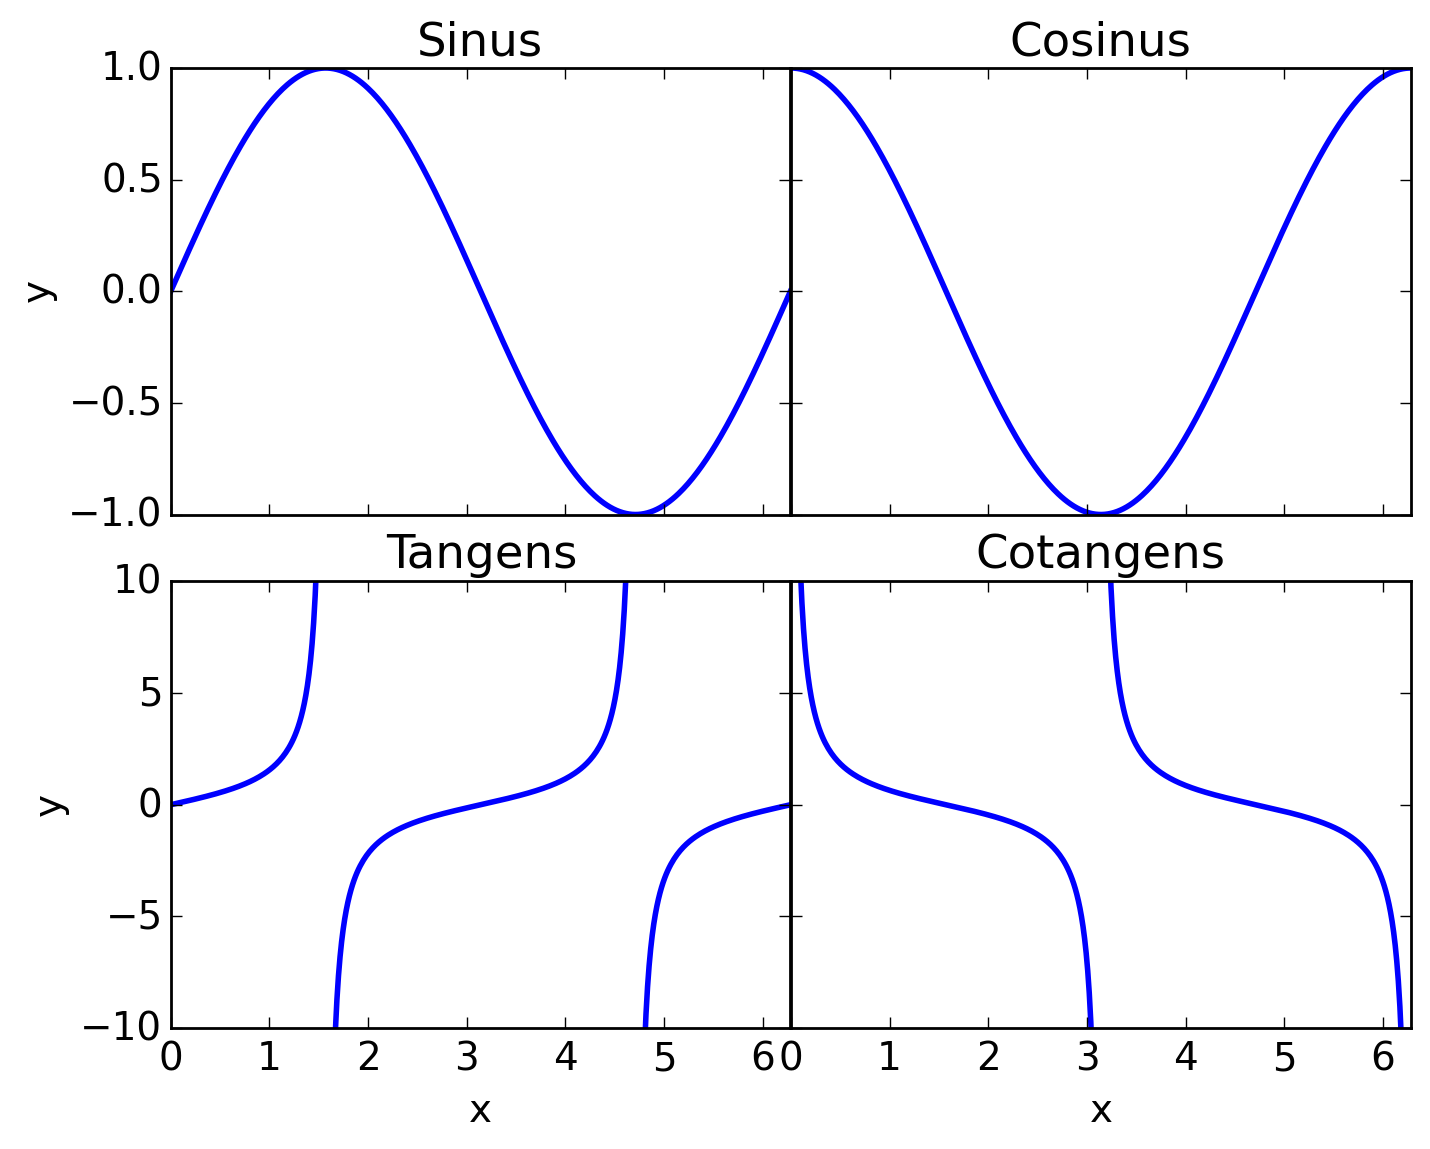
\includegraphics[width=0.9\textwidth]{trigo_funktionen}
  \caption{Trigonometrische Funktionen: Gezeigt sind die Sinusfunktion
    (oben links), die Cosinusfunktion (oben rechts), der Tangens
    (unten links) und der Cotangens (unten rechts).}
  \label{fig:trigo_funk}
\end{figure}
%
\section{Kreis und Quadrat}
Ein Kreis ist eine ebene geometrische Figur. Er wird definiert als die
Menge aller Punkte einer Ebene, die einen konstanten Abstand zu einem
vorgegebenen Punkt dieser Ebene (dem Mittelpunkt) haben. Der Abstand
der Kreispunkte zum Mittelpunkt ist der Radius oder Halbmesser des
Kreises, er ist eine positive reelle Zahl. Der Kreis gehört zu den
klassischen und grundlegenden Objekten der euklidischen Geometrie.

In der Geometrie ist ein Quadrat (veraltet auch Geviert) ein
spezielles Polygon, nämlich ein ebenes, konvexes und regelmäßiges
Viereck.

Kreis und Quadrat sind in \figureref{fig:kreis_quadrat}
\emph{korrekt} dargestellt.
%
\begin{figure}[ht]
  \centering
  % Wir fassen zwei Figuren zu einer zusammen. Damit so nebeneinander
  % gesetzt werden darf die Gesamtbreite der Figuren '\textwidth'
  % nicht überschreiten.
  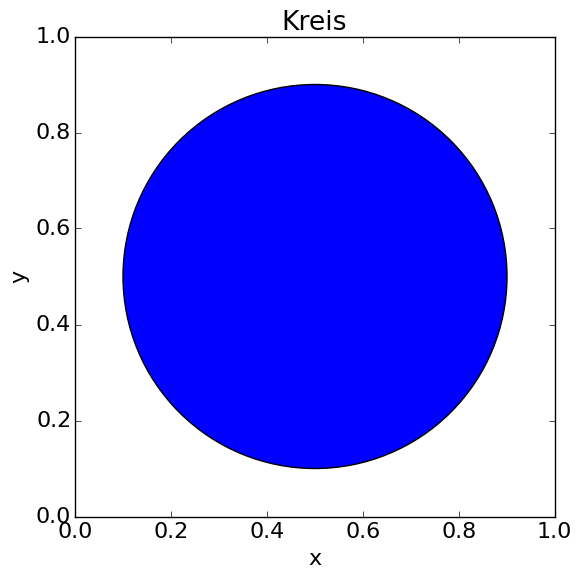
\includegraphics[width=0.45\textwidth]{kreis}
  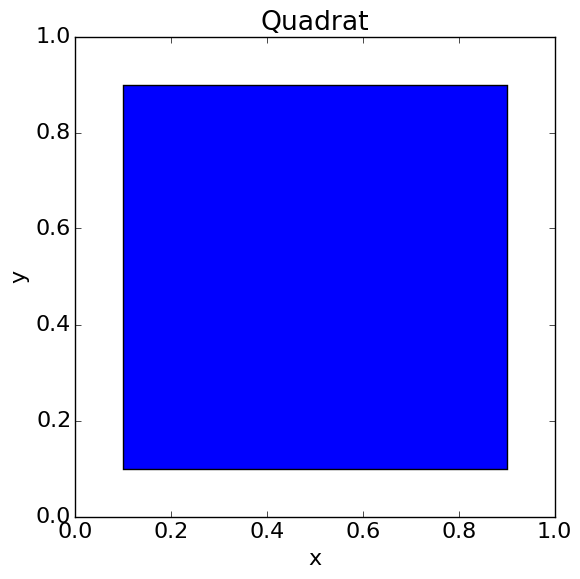
\includegraphics[width=0.45\textwidth]{quadrat}
  \caption{Kreis (links) und Quadrat(rechts) mit korrekter Skalierung}
  \label{fig:kreis_quadrat}
\end{figure}
%
